% vim:ts=4:sw=4
% Copyright (c) 2014 Casper Ti. Vector
% Public domain.

\chapter{相关工作}
\section{主要相关技术调研}
\subsection{crawler}
\subsubsection*{Beatifulsoup}
Beautiful Soup提供一些简单的、python式的函数用来处理导航、搜索、修改分析树等功能。它是一个工具箱,通过解析文档为用户提供需要抓取的数据,因为简单,所以不需要多少代码就可以写出一个完整的应用程序。Beautiful Soup自动将输入文档转换为Unicode编码,输出文档转换为utf-8编码。你不需要考虑编码方式,除非文档没有指定一个编码方式,这时,Beautiful Soup就不能自动识别编码方式了。然后,你仅仅需要说明一下原始编码方式就可以了。Beautiful Soup已成为和lxml、html6lib一样出色的python解释器,为用户灵活地提供不同的解析策略或强劲的速度
\subsection{人脸识别技术}
人脸识别是一项热门的计算机技术研究领域,它属于生物特征识别技术,是对生物体(一般特指人)本身的生物特征来区分生物体个体。生物特征识别技术所研究的生物特征包括脸、指纹、手掌纹、虹膜、视网膜、声音(语音)、体形、个人习惯(例如敲击键盘的力度和频率、签字)等,相应的识别技术就有人脸识别、指纹识别、掌纹识别、虹膜识别、视网膜识别、语音识别(用语音识别可以进行身份识别,也可以进行语音内容的识别,只有前者属于生物特征识别技术)、体形识别、键盘敲击识别、签字识别等。
\subsubsection*{Face++}
Face++是新一代云端视觉服务平台,提供一整套世界领先的人脸检测,人脸识别,面部分析的视觉技术服务。
Face++旨在提供简单易用,功能强大,平台通用的视觉服务,让广大的Web及移动开发者可以轻松使用最前沿的计算机视觉技术,从而搭建个性化的视觉应用。Face++同时提供云端REST API以及本地API(涵盖Android, iOS, Linux, Windows, Mac OS),并且提供定制化及企业级视觉服务。通过Face++,您可以轻松搭建您自己的云端身份认证,用户兴趣挖掘,移动体感交互,社交娱乐分享等多类型应用。
face++提供了相应的http请求的接口,并提供了python,java,c++的API接口。在本项目中,作者对于face++对于nodejs的api接口进行了补全,能够很好的支持nodejs对于face++的接口应用,方便之后的nodejs开发者能够有效的利用该项技术。

\subsubsection*{caffe}
Caffe( http://caffe.berkeleyvision.org/ )是一个清晰而高效的深度学习框架,其作者是博士毕业于UC Berkeley的贾扬清(http://daggerfs.com/ ),他目前在Google工作。Caffe是纯粹的C++/CUDA架构,支持命令行、Python和MATLAB接口;可以在CPU和GPU直接无缝切换。caffe在图像处理方面有着自己独特的效果。


而比较了这两项技术之后,由于face++是专门做人脸识别的技术,他的各项评测也遥遥领先,所以在本文准备使用face++的API来实现应用。
\subsubsection*{Face++的API接口}
\begin{figure}[h]
\begin{minipage}[t]{0.45\linewidth}
\centering
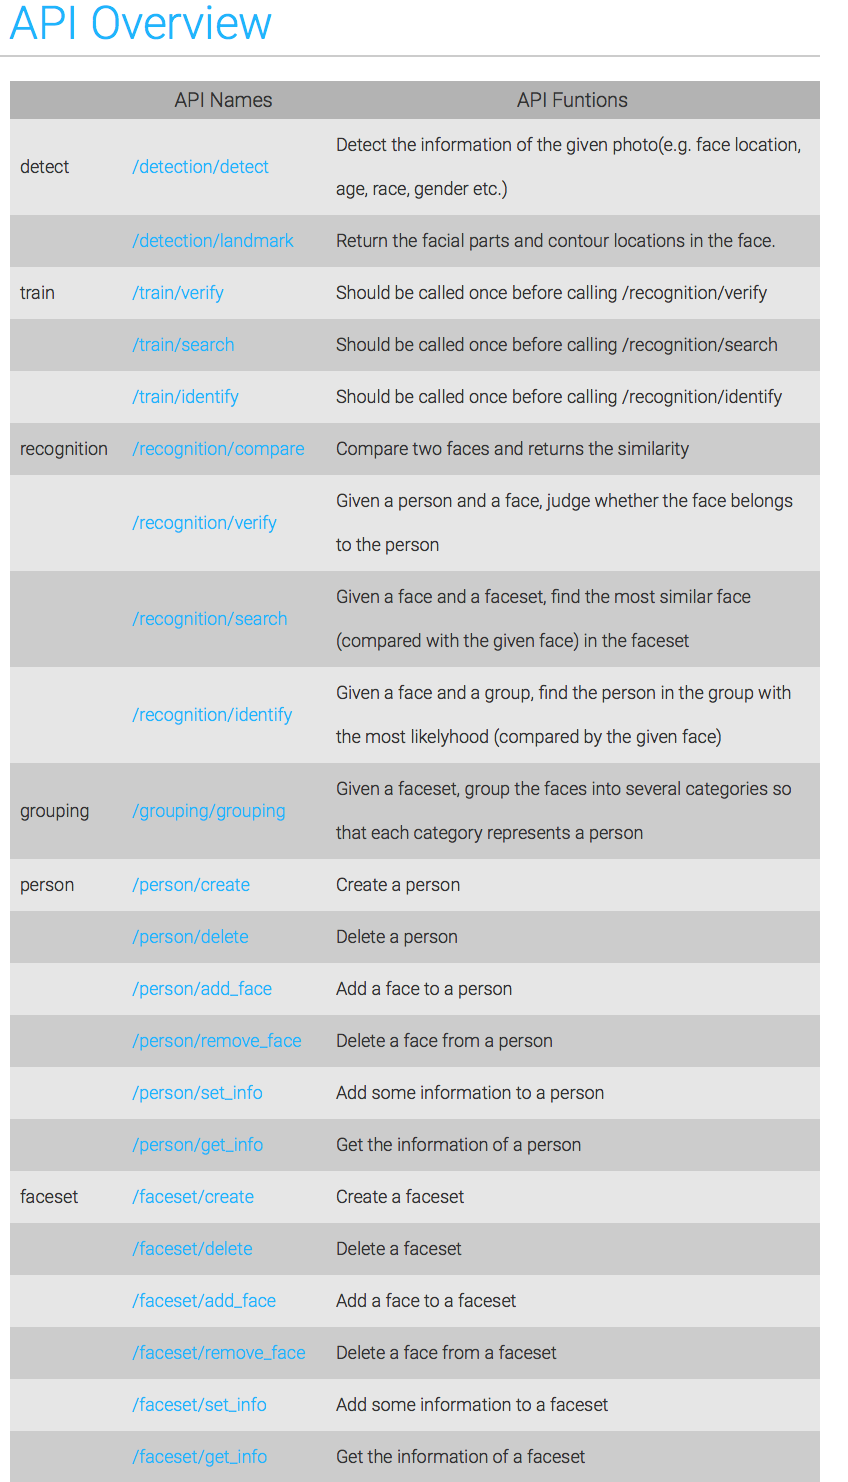
\includegraphics[width=\textwidth]{img/chap2/Face++API.png}
\caption{Face++API\label{Face++API}}
\end{minipage}

\begin{minipage}[t]{0.45\linewidth}
\centering
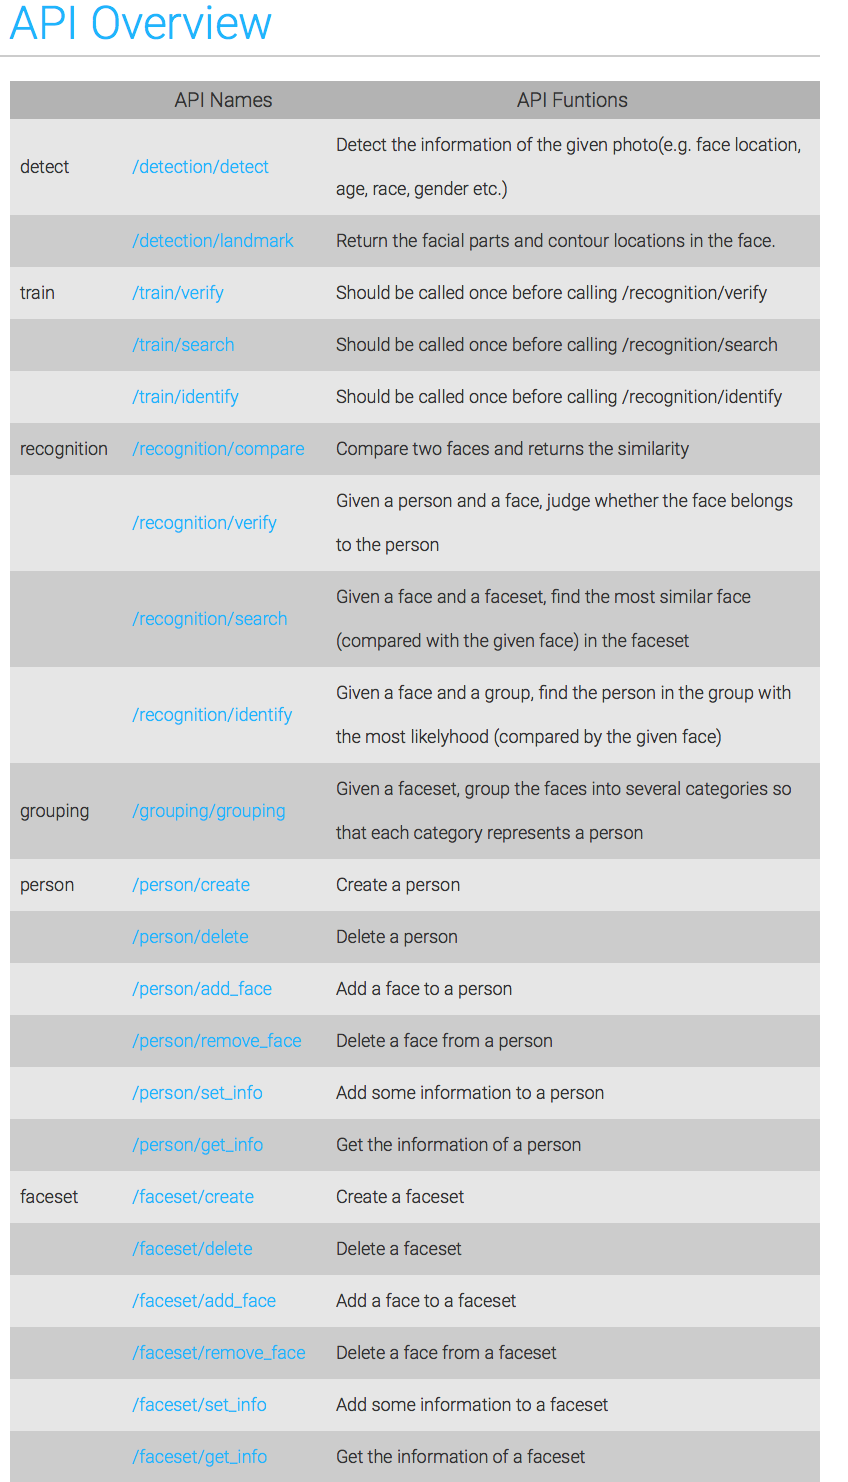
\includegraphics[width=\textwidth]{img/chap2/Face++API.png}
\caption{Face++API\label{Face++API}}
\end{minipage}

\end{figure}


\subsection{移动应用}
移动应用(Mobile application)安装和运行在移动设备上。它随着智能手机的推出,由于其移动性和娱乐性,在近年来达到了全新的巅峰。目前有三大主流的移动应用平台,分别为IOS,Android和Windows Phone。据三大平台统计,从2010年到2013年,移动应用的数目增加了100多万个。因此,移动应用是目前软件开发的一种最流行的模式,移动设备庞大的用户量和较小的开发经费也吸引了越来越多的自由开发者加入到了移动应用的开发者行列之中。
\subsubsection{angularJS}
ngularJS是一款开源JavaScript函式庫,由Google维护,用來協助單一頁面應用程式運行的。它的目标是透過MVC模式(MVC)功能增强基于浏览器的应用,使开发和测试变得更加容易。
函式庫讀取包含附加自定義(標籤屬性)的HTML,遵從這些自定義屬性中的指令,並將頁面中的輸入或輸出與由JavaScript變量表示的模型綁定起來。這些JavaScript變量的值可以手工設置,或者從靜態或動態JSON資源中獲取。
AngularJS是建立在這樣的信念上的:即声明式编程應該用於構建用戶界面以及編寫軟件構建,而指令式編程非常適合來表示業務邏輯。[1]框架採用並擴展了傳統HTML,通過雙向的數據綁定來適應動態內容,雙向的數據綁定允許模型和视图之間的自動同步。因此,AngularJS使得對DOM的操作不再重要並提升了可測試性。
設計目標:
將應用邏輯與對DOM的操作解耦。這會提高代碼的可測試性。
將應用程序的測試看的跟應用程序的編寫一樣重要。代碼的構成方式對測試的難度有巨大的影響。
將應用程序的客戶端與服務器端解耦。這允許客戶端和服務器端的開發可以齊頭並進,並且讓雙方的復用成為可能。
指導開發者完成構建應用程序的整個歷程:從用戶界面的設計,到編寫業務邏輯,再到測試。
\subsubsection{ionic}
Ionic提供了一个免费且开源的移动优化HTML,CSS和JS组件库,来构建高交互性应用。基于Sass构建和AngularJS 优化,并形成了一个强大的 HTML5 应用程序开发框架,可以帮助您使用 Web 技术,比如 HTML、CSS 和 Javascript 构建接近原生体验的移动应用程序。Ionic 主要关注外观和体验,以及和你的应用程序的 UI 交互,特别适合用于基于 Hybird 模式的 HTML5 移动应用程序开发。且它是一个轻量的手机UI库,具有速度快,界面现代化、美观等特点。为了解决其他一些UI库在手机上运行缓慢的问题,它直接放弃了IOS6和Android4.1以下的版本支持,来获取更好的使用体验.


Ionic是现在GitHub上的最火的开源项目之一,具有超过16,000星及以上创建600000Ionic app。Ionic遵循视图控制模式,通俗的理解和 Cocoa 触摸框架相似。在视图控制模式中,我们将界面的不同部分分为子视图或包含其他视图的子视图控制器。然后视图控制器“驱动”内部视图来提供交互和UI功能。一个很好的例子就是标签栏(Tab Bar)视图控制器处理点击标签栏在一系列可视化面板间切换。
由于ionic在三大平台都能够使用,存在了很强大的适应性,并且针对于现有先进的移动设备.

\subsection{数据库调研}
\subsubsection{来源}
根据本文所要实现的应用的特性,是基于人脸的社交应用,而无疑最符合这个性质的社交应用就是婚恋市场的社交应用,而也只有婚恋的用户才会在大概率上将他们的真实人物照片提交到应用上,为了模拟这个应用的特性,本文实验的数据库的来源也需要从类似的网站上抓取,排除掉国外的婚恋网站,作为国内的比较流行的婚恋网站有,百合网,珍爱网,世纪佳缘。


通过比较这几个网站的数据,发现百合网的会员资料的开放程度不及世纪佳缘,珍爱网。而世纪佳缘的用户活跃度和注册数远远优于珍爱网。所以本文拟用世纪佳缘的数据作为本文应用的数据库来源。
\subsubsection{mongodb}
Mongo DB 是目前在IT行业非常流行的一种非关系型数据库(NoSql),其灵活的数据存储方式备受当前IT从业人员的青睐。Mongo DB很好的实现了面向对象的思想(OO思想),在Mongo DB中 每一条记录都是一个Document对象。Mongo DB最大的优势在于所有的数据持久操作都无需开发人员手动编写SQL语句,直接调用方法就可以轻松的实现CRUD操作。
MongoDB的文档模型自由灵活,可以让你在开发过程中畅顺无比。对于大数据量、高并发、弱事务的互联网应用,MongoDB可以应对自如。MongoDB内置的水平扩展机制提供了从百万到十亿级别的数据量处理能力,完全可以满足Web2.0和移动互联网的数据存储需求,其开箱即用的特性也大大降低了中小型网站的运维成本。

% % 中文测试文字。
% \pkuthssffaq

